\documentclass[orivec]{llncs}
\usepackage{graphicx}
\usepackage{amsmath}			% for "cases"
\usepackage{amsfonts}		% for frakur fonts
\usepackage{mathrsfs}		% for curly "E" error symbol
\usepackage{float}
\usepackage{tcolorbox}		% for wrapping example in color box
\usepackage{wrapfig}			% wrap figure beside text, used in example
\usepackage{tikz-cd}			% commutative diagrams
\usepackage{amssymb}			% for \multimap, \updownarrow, \bigstar
\usepackage{sectsty}			% change section color
\usepackage{turnstile}		% longer turnstiles
\usepackage{hyperref}		% include web link for RL sample code
\usepackage[normalem]{ulem}	% underline unbroken with \uline

\usepackage{geometry}		% change paper size
\geometry{
  a4paper,         % or letterpaper
  textwidth=18cm,  % llncs has 12.2cm
  textheight=24cm, % llncs has 19.3cm
  heightrounded,   % integer number of lines
  hratio=1:1,      % horizontally centered
  vratio=2:3,      % not vertically centered
}
\usepackage[fontsize=14pt]{scrextend}

% *************** Delete when not using Chinese or colors **********************
%\usepackage{xeCJK}
%\setCJKmainfont[BoldFont=SimHei,ItalicFont=KaiTi]{SimSun}
\usepackage{color}
\definecolor{Cerulean}{RGB}{100,100,200}
%\newcommand{\emp}[1]{\textbf{\textcolor{Cerulean}{#1}}}
\newcommand{\emp}[1]{\textbf{#1}}
\definecolor{grey}{rgb}{0.9,0.9,0.9}  % grey

% \chapterfont{\color{blue}}  % sets colour of chapters
\sectionfont{\color{blue}} 
\subsectionfont{\color{blue}} 
\subsubsectionfont{\color{blue}} 

\newcommand{\vect}[1]{\boldsymbol{#1}}
\newcommand*\sigmoid{\vcenter{\hbox{\includegraphics{sigmoid.png}}}}
\newcommand*\KB{\vcenter{\hbox{\includegraphics{KB-symbol.png}}}}
\newcommand*\invsigmoid{\vcenter{\hbox{\includegraphics{inverse-sigmoid.png}}}}
\newcommand{\invW}{\, \rotatebox[origin=c]{90}{W}}
\newcommand{\invw}{\, \rotatebox[origin=c]{90}{w}}
\newcommand*\rectifier{\vcenter{\hbox{\includegraphics{rectifier.png}}}}
\newcommand{\dashh}{\textemdash~}
\newcommand{\code}[1]{{\footnotesize{\ttfamily #1}}}
\newcommand{\tab}{\hspace*{1cm} }

% ***** Boxed variables inside math equations
% \newcommand*{\boxedcolor}{black}
\makeatletter
% \renewcommand{\boxed}[1]{\textcolor{\boxedcolor}{%
% \fbox{\normalcolor\m@th$\displaystyle#1$}}}
% \setlength{\fboxsep}{1pt}
\renewcommand{\boxed}[1]{\fbox{\m@th$\displaystyle\scalebox{0.9}{#1}$} \,}
\makeatother

\overfullrule=0mm

\newsavebox{\MyName}
\savebox{\MyName}{\includegraphics[scale=0.6]{YKY.png}}

\title{Reinforcement learning tutorial}
\titlerunning{RL tutorial}
\author{\usebox{\MyName} (King-Yin Yan)
% \\ \footnotesize{General.Intelligence@Gmail.com}
}
\institute{General.Intelligence@Gmail.com}

\begin{document}

\maketitle
\setlength{\parindent}{0em}
% \setlength{\parskip}{2.8ex plus0.8ex minus0.8ex}
\setlength{\parskip}{2.8ex}

%\begin{abstract}
%简单介绍强化学习。
% 假设 $x$ 是思维状态。 在经典逻辑智能中,$x$ 是一束命题,代表当下的思考状况。 思考的过程就是不断重复进行推导: $x \vdash x' \vdash ...$。 在经典 AI 中这个作用是靠无数的逻辑 rules 来达成的。 但现在我们的做法是将 $x$ 放到向量空间中,再用一个 recurrent 神经网络来取代整个 rules base。
%\end{abstract}

\setcounter{section}{-1}
\section{What is reinforcement learning?}

\textbf{Reinforcement learning} is a branch of machine learning that is particularly suitable for controlling an \textbf{autonomous agent} who interacts with an \textbf{environment}.  It uses \textbf{sensory perception} and \textbf{rewards} to continually modify its \textbf{behavior}.

When you hear reinforcement learning, it should invoke an imagery in your mind of a little critter such as this cockroach: $\vcenter{\hbox{\includegraphics[scale=0.5]{cockroach.png}}}$

As for the idea of an \textbf{environment}, you should think of a maze such as in this: classic game:\begin{equation}
\includegraphics[scale=0.8]{pacman-0.png}
\end{equation}
that includes some monsters chasing after you, some food that you could eat to increase your score (these represent negative and positive rewards).  Of course, in real applications the ``environment'' and ``rewards'' can be abstract;  This game is just a concrete example.

\section{What goes in and out?}

Keep in mind, the \textbf{inputs} to the reinforcement learning algorithm are the following:\let\labelitemi\labelitemii
\begin{itemize}
\item \underline{S}tates = the environment \\
For example: each square in the maze is a state
\item \underline{A}ctions = under each state, which actions are allowed?
\item \underline{R}ewards =  upon visiting each new state, there is an associated positive or negative \textbf{utility}
\end{itemize}
And the output of the algorithm is:
\begin{itemize}
\item \underline{P}olicy = under each state, which action would you choose?
\end{itemize}
So this 4-tuple $(S, A, R, P)$ constitutes a reinforcement learning system.  In abstract algebra, we often use such \textbf{tuples} to define systems or structures.

A more concrete example is:
\begin{itemize}
\item states $S$ =  each square of the maze, which can be represented by its coordinates, eg (1,3)
\item actions $A$ = on each square of the maze, you can go either $\{ \uparrow, \downarrow, \leftarrow, \rightarrow \}$
\item rewards $R$ = under the current state, the square of the maze may contain food (+1) or a monster (-100)
\item policy $P$ = a \textbf{function} from states $\rightarrow$ actions, ie, given any state, it returns with an action.

\end{itemize}
$(S, A, R)$ are defined by the user, $P$ would be automatically calculated by the algorithm.

\section{Between men and insects}

The first question that comes to mind:  why not just use this technique to build strong AI?  But the current state of the art of reinforcement learning can only handle relatively small and simple environments, it is still rather helpless when faced with larger and more complex worlds, such as the $10^{\mbox{xxx}}$ state space of chess.

The key lies in the fact that, higher intelligent beings build up knowledge or \textbf{world models} in their brains, whereas naive reinforcement learning is only concerned with state-action pairs.

The leading researcher in reinforcement learning, Richard Sutton, thinks that RL is the only learning technique that takes into consideration elements such as autonomous agents, environments, and rewards, therefore it should be the \textbf{top-level architecture} in an AI system, where other modules such as logic and pattern recognition should subsume under its control.  I think this makes a lot of sense.
\begin{equation}
\includegraphics[scale=0.4]{Richard-Sutton.jpg}
\end{equation}

Thus to build a strong AI, a possible scheme is to combine reinforcement learning with a certain ability to handle complex world models:
\begin{equation}
\includegraphics[scale=0.7]{cockroach-KB-person.png}
\end{equation}

\noindent ``\textit{You have made your way from worm to man, but much in you is still worm.}''

\hfill --- Nietzsche, \textit{Thus spoke Zarathustra}

\noindent ``\textit{If men cease to believe that they will one day become gods then they will surely become worms.}''

\hfill --- Henry Miller

\section{Code}

Learning AI is boring without programs.  Here is a simple demo that I found on the web, the author is Travis DeWolf:

\href{https://studywolf.wordpress.com/2012/11/25/reinforcement-learning-q-learning-and-exploration/}{https://studywolf.wordpress.com/2012/11/25/reinforcement-learning-q-learning-\\
and-exploration/}

It only requires \textbf{Python} to run, but you may need to install \textbf{PyGame} first.

{\color{red} Cat}, {\color{blue} mouse}, {\color{yellow} cheese}:
\begin{equation}
\includegraphics[scale=0.25]{RL-demo.png}
\end{equation}

The cat's behavior is simply to move towards the mouse (this is without intelligence), the mouse's behavior is learned by the algorithm.

Note that, in the main program and in \textbf{cellular.py}, the behavior of the maze world is defined, but this is purely a game program that has no intelligence in it.  You can use $\{ \uparrow, \downarrow, \leftarrow, \rightarrow \}$ to control the agents' movements, and that's all of it.

The reinforcement learning algorithm is in qlearn.py, which is very short, and the actual learning code is essentially just one line, that is:

\tab \code{def learnQ(self, state, action, reward, value): }\\
\tab \code{oldv = self.q.get((state, action), None) }\\
\tab \code{if oldv is None:} \\
\tab \code{\tab self.q[(state, action)] = reward }\\
\tab \code{else: }\\
\tab \code{\tab \textcolor{red}{self.q[(state, action)] = oldv + self.alpha * (value - oldv) }}

Just this one line of code, is able to make the mouse avoid the cat, and eat the cheese.  It will be explained below...

\section{How does RL work?}

Chapter 21 of \textit{AI: a modern approach} has a very good introduction to RL.  \textit{AIMA} is of course the classic AI textbook, many people say that they love AI after studying this book.  The strength of this book is that it uses plenty of words to explain all concepts and principles patiently, so the reader would not feel disorganized.  For example, Chapter 21 first explains passive reinforcement learning, which means to hold the policy fixed, and then simply calculate the agent's expected utility (ie the total rewards).  Having established this foundation then we compare different policies.  This way of thinking is very common in mathematics:  First consider a case so simple that any idiot can solve, and then gradually introduce more complexity.  For example in mathematical induction, to move from case $N=1$ to  $N \rightarrow \infty$.

To avoid repeating the book, I will just explain the minimum knowledge required to understand $Q$ learning.

\section{Utility}

$U$ is the sum of rewards after a sequence of actions.  For example, the utility of playing one chess move is not just the immediate reward of that move, but also includes the consequences after that move.  For example, a player may greedily eat a pawn, but then got checkmated 10 moves later.  Or, faced with delicious food, some people may choose not to eat, for fear of getting fat.

The \textbf{utility} of a state is:  assuming the policy is fixed, and considering all possible future transitions starting from this state, the average expectation of the total reward:

$$ U(S_0) = \mathbb{E}[ \; \sum_{t=0}^{\infty} \; \gamma^t \; R(S_t) \; ] $$
where $\mathbb{E}[]$ is expectation value, $\gamma$ is the discount factor, such as 0.9 or something.

Real example:  consider a maze like this one:
\begin{equation}
\includegraphics[scale=0.4]{RL-simple-maze.png}
\end{equation}

The arrows represent one policy out of many possible policies.

According to this policy, starting from $(1,1)$ we may get this \textbf{outcome}:
\begin{equation}
\includegraphics[scale=0.7]{RL-state-transition-eg-1.png}
\end{equation}

The orange number below is the \textbf{reward} for each state.  In this example, every square that is not the goal, will have 0.04 deducted from the score.

However, even starting from the same state, using the exact same policy, can give different outcomes.  For example, when the creature tries to crawl left from $(1,3)$, the actual outcome may be falling one square downwards.  Such \textbf{state transitions} are dictated by probabilities from the external world.  (For example, someone gets a university degree, but the economy falls into recession, his actual salary may not be as high as he has expected).

Another outcome of the same policy could be:
\begin{equation}
\includegraphics[scale=0.7]{RL-state-transition-eg-2.png}
\end{equation}
or this:
\begin{equation}
\includegraphics[scale=0.7]{RL-state-transition-eg-3.png}
\end{equation}

\section{Bellman condition}

The Bellman optimality condition is the \textit{central idea} in \textbf{dynamic programming}.

The artificial intelligence community calls it \textbf{reinforcement learning}, but in control theory it is called \textbf{dynamic programming};  the two are synonymous.  Richard Bellman in 1953 proposed this equation, while he was working at RAND corporation, dealing with operations research problems.  He also coined the phrase "curse of dimensionality" to describe the major obstacle in dynamic programming.

The problem we try to solve is:  to make a series of \textbf{sequential decisions}.

The Bellman condition says:  ``\uline{if we cut off a tiny bit from the endpoint of the optimal path, the remaining path is still an optimal path between the new endpoints}.''

In other words, if we have made a sequence of optimal decisions A B C D E..... then this sequence, with the endpoint A removed, = B C D E ..... is still an optimal decision sequence when applied to the rest of the states.

(For example, you plan to drive from Los Angeles to New York:
$$ \mbox{Los Angeles} \rightarrow \mbox{Las Vegas} \rightarrow ... ... \rightarrow \mbox{New York} $$
and you have chosen the cheapest route, which passes through 6 stops, the 2nd stop being Las Vegas.  Now if you remove the starting point Los Angeles, then the remaining route:
$$ \mbox{Las Vegas} \rightarrow ... ... \rightarrow \mbox{New York} $$
would still be the cheapest route for the remaining stops.)

Mathematically:
$$ U^*(S) = \max_a \{ R(a) + U^*(S') \} \quad \quad \mbox{or,} $$
$$ U^*(\mbox{whole path}) = \max_a \{ R(\mbox{choose action $a$ in current state}) + U^*(\mbox{rest of path}) \} $$
$*$ denotes \emp{optimal}. This seemingly simple formula is the \uline{entire content} of dynamic programming;  What it means is that:  When seeking the path with the best value, we cut off a bit from the path, thus reducing the problem to a smaller problem;  In other words, it is a \textbf{recursive relation} over time.

\section{Delta rule}

This is just a simple trick, appearing often in machine learning.  Suppose we have an \textbf{ideal} value, we want to gradually adjust the \textbf{current} value so that it asymptotically \textbf{approaches} this ideal.  What we do is:
$$ \mbox{current value} := \mbox{current value} + \alpha ( \mbox{ideal value} - \mbox{current value}) $$
where $\alpha$ is called the ``learning rate''.  ``Delta'' ($\Delta$) referes to the \textbf{difference} between the ideal and current values.

Obviously, as we repeatedly perform the above step, the current value will get closer and closer to the ideal value.

(The \textbf{differential} version of the Delta rule is the familiar \textbf{gradient descent} algorithm:  $x \mbox{ += } \eta \cdot \frac{dy}{dx} \,$ )

\section{Temporal difference (TD) learning}

Applying the Delta rule on the Bellman equation to find the optimal path, we get what is called \textbf{temporal difference} learning.

Again we start with the simple case:  assume policy is fixed, the aim is to learn the utility of all states.

\textbf{Ideally}, the value of $U(S)$ can be obtained by:  starting from state $S$, trying all possible state transitions, summing the total rewards along these paths, and finding the average total reward among all paths.

But in reality, our agent can only experience \uline{one} state transition after each action.

So we need to apply the Bellman condition:  The $U$ value of a state $S$ is equal to:  its own reward, added with the $U$ values of all possible subsequent states, taking the probabilistic average (ie expectation value), and multiplying with the discount factor $\gamma$:
$$ U(S) = R(S) + \gamma \sum_{S'} P(S \rightarrow S') \; U(S') $$
where $P$ is the transition probability, $S'$ is the subsequent state, $\sum$ is the summation over all subsequent states.  In other words, this is a relation between the ideal $U(S)$ and $U(\mbox{subsequents of }S)$, as a \textbf{recursive relation}.

For example, assume the agent's estimations of state (1,3) and state (2,3) are respectively 0.84 and 0.92.  Also the agent observes that under the current policy, the transition from (1,3) to (2,3) always occurs.  Then the $U$ values of these 2 states should satisfy this constraint:
$$ U(1,3) = -0.04 + U(2,3) $$
In other words, this is the \textbf{local constraint} on the $U$ values between 2 states.

The idea of TD learning:  assume other $U(S')$ estimates are correct, use the Bellman optimality constraint to \textbf{adjust} the $U(S)$ of the current state.  As the number of trials grows large, all the $U$ estimates will approach ideal.  The agent only needs to use this update rule:
$$ U(S) \mbox{  +=  } \alpha ( \; R(S) + \gamma U(S') - U(S) \; ) $$

$\alpha$ is the \textbf{learning rate}, it determines the speed of learning (but it cannot be too large, lest \textbf{overshooting} may occur).  The stuff after $\alpha$ is the difference between the current estimated $U(S)$ and the $U(S)$ estimated using ideal constraints.  For the ideal $U(S)$ and $U(S')$, this difference would be 0.  Whereas for each time step, we just use $\alpha$ to \textbf{partially} adjust this difference.

Lastly I should mention that, in the above equation of the ideal constraint, there is a summation over all probabilities $P$, but the $P$ disappeared in the update formula.  That is because the agent is acting in the environment, and this \textit{implicitly} performs a \textbf{sampling} of the state transition probabilities.  In other words, the summation is performed by the agent itself.

$P$ is the probabilities of state transitions, in other words a \textbf{model} of the world.  TD learning does not need to learn $P$, that is why it is called \textbf{model-free} learning.  But just as we have said in the beginning, model-free is not necessarily a good thing.  Human intelligence lies in the fact that we do have some pretty good models of the external world.

\section{Q value}

$Q$ value is just a variation of $U$ value;  there is a $U$ value for each state, and $Q$ is the \textbf{decomposition} of $U$ by all the actions in that state.  In other words, $Q$ is the utility of doing action $A$ in state $S$.

The relation between $Q$ and $U$ is:
$$ U(S) = \max_A  Q(A, S) $$

What is $Q$ good for?  Below we will introduce \textbf{active} learning, and $Q$ values, when combined with TD learning, can eliminate $P$ in active learning, thus achieving the model-free effect.

The update rule (in the last section) needs only be revised with this new rule:
$$ U(S) \mbox{  +=  } \alpha ( \; R(S) + \gamma \max_{A'}  Q(A', S') - Q(A, S) \; ) $$

\section{Active learning}

In passive learning, with the policy fixed, we can already calculate the utility $U(S)$ for each state $S$, or the utility $Q(S,A)$ of doing action $A$ under each state $S$.

If the policy can change, we just need to calculate the $Q$ values for different policies, then choose the action $A$ corresponding to the maximum $Q$ value in each state, that would be the best policy, right?

When we actually execute the above, we find that the agent's policies are really bad!  The reason being that, during the learning process, the $Q$ values are estimates rather than ideals, and if we act according to such $Q$'s, the agent becomes very \textbf{short-sighted}, and fails to find the optimal policy.  (For example, a person always goes to the same restaurant, but if he walks a different path, he could find a much better restaurant.)

The agent needs to try some unknown states or actions in order to learn the optimal policy;  This is the so-called \textbf{exploration} vs \textbf{exploitation} trade-off.

The way to do this, is to artificially increase the utilities of unknown states:
$$ U(S) = R(S) + \gamma \max_A \mathcal{F}[ \; \sum_{S'} P(S \rightarrow S') U(S'), \; N(A, S) \; ] $$
where $N(A, S)$ is the number of times the combination of state $S$ and action $A$ has occurred (= has been experienced), $\mathcal{F}$ is the exploration function, it normally returns the estimate of $U$, but when $N$ is small (that means we have little experience of $S$, $A$), it will return a relatively larger estimate, which represents the utility of ``curiosity''.

% 结语

% 本来想写一篇人人能读懂的 RL 简介,但发觉写到长篇大论才勉强解释完。  希望女朋友能读懂 :)

%\section*{Acknowledgements}

\bibliographystyle{plain} % or number or aaai ...
\bibliography{AGI-book}

\end{document}
